\documentclass[10pt]{article}
\usepackage[margin=1in]{geometry}
\usepackage[T1]{fontenc}
\usepackage{lmodern}
\usepackage{graphicx,booktabs,amsmath,amssymb,caption,float}
\usepackage[hidelinks]{hyperref}
\captionsetup{font=small,labelfont=bf}
\setlength{\parskip}{3pt}
\newcommand{\nats}{\,nats}

\title{Does staggering update frequency reduce catastrophic forgetting?\\
\large A pre-registered negative result in small transformers}
\author{Project \texttt{catadye}\\ \small Code, data and raw results: \url{https://github.com/sykeriin/catadye}}
\date{November 2026}

\begin{document}
\maketitle

\begin{abstract}
Google's Nested Learning paper proposes a Continuum Memory System (CMS): MLP blocks that update at different
frequencies. Its authors report reduced forgetting, but I found no independent test of whether the frequency
staggering itself is responsible. I test that component in isolation, in a plain transformer, with the hypotheses,
metrics and decision rule committed before each experiment. The main comparison is against an \emph{LR-matched
control}: the same blocks updated every step at a proportionally smaller learning rate, because under Adam a block that updates
every $k$ steps moves roughly $1/k$ as far. Two training-time pilots (16--24M parameters, TinyStories then Python
code, 3 seeds) find no reduction in forgetting at matched plasticity: CMS forgets $+0.09$ nats more than the baseline
(95\% CI $[-0.17,+0.25]$) against a pre-registered bar of a 10\% reduction. A test-time probe, closer to the paper's mechanism,
shows that staggered updates forget 8--31\% less than single-rate updates at the same learning rate, but the LR-matched control forgets
8--11\% less than staggering. Post-hoc drift measurements show that the staggered blocks do move far less (up to $50\times$)
while forgetting is unchanged, so the forgetting is carried by parts of the network that update every step. The
experiments do not test Hope's nested consolidation, self-modifying memory, multi-timescale momentum, or
pretrained backbones, and they are small (3 seeds, $\leq$24M parameters).
\end{abstract}

\section{Introduction}
Catastrophic forgetting, the loss of earlier capabilities when a network trains on new data, remains a central obstacle to
continually updated language models. Nested Learning~\cite{nl} reframes architectures and optimizers as nested
associative memories that update at different frequencies, and proposes Hope, which combines a self-modifying Titans-style
memory, multi-timescale momentum and a Continuum Memory System (CMS). The authors report reduced forgetting while stating that
forgetting is not solved in general. No official code was released; community reimplementations state that they target
mechanism-level fidelity and do not claim parity with the paper's numbers~\cite{kmccleary}.

The paper's evidence for each component is thin where forgetting is concerned. Its component ablation (Table~6)
measures language-modelling perplexity and reasoning accuracy, not forgetting; the multi-timescale momentum optimizer (M3) is evaluated on
loss and training efficiency, not forgetting; and the continual-learning results use pretrained Llama-3 backbones after 15B tokens of extra
pre-training. A keyword-filtered scan of the papers citing it (106 on Semantic Scholar in November 2026), plus web searches, turned up
extensions, applications and optimizer variants but no replication or component ablation of the forgetting claims.
That absence is a finding of my search, not a proof that none exists.

\textbf{Research question.} Does staggering update frequency alone reduce forgetting in a plain small transformer, and is any
gain distinguishable from simply taking smaller steps? This is deliberately a narrow question. It isolates the cheapest component of Hope,
and the answer does not decide whether Hope works.

\textbf{Contributions.} (i) A pre-registered design with an LR-matched control and a matched-plasticity comparison, so that
slower learning is not mistaken for less forgetting. (ii) Two training-time pilots and a test-time probe, all negative with respect to the pre-registered
criteria. (iii) A post-hoc drift analysis explaining why. (iv) Disclosure of the limits, including run-to-run nondeterminism on the
GPU that is as large as the effects discussed.

\section{Related work}
\textbf{Nested Learning and Hope}~\cite{nl} (above). \textbf{Titans Revisited}~\cite{titans} reimplements the Titans neural
memory and finds that the memory helps relative to attention-only models but that memory updates alone are insufficient for meaningful test-time
learning when the backbone is frozen, a caution that applies to the test-time probe here.
\textbf{Forgetting in language models.} Work on spurious forgetting finds that freezing bottom layers reduces loss of earlier
behaviour~\cite{spurious}; an optimizer study (in a vision-style setup) finds lower layers prefer smaller learning rates~\cite{resampling}; and a 2026 mechanistic preprint reports reduced forgetting when attention
weights are frozen during fine-tuning~\cite{mech}. These are the closest relatives of per-block step-size control and motivate
the LR-matched control. \textbf{Multi-timescale learning.} Fast/slow weight schemes are an old idea; recent work pairs slow parameters with fast
context~\cite{fastslow}. I found no prior application of per-block update periods to forgetting in language-model domain sequences,
though my search was not exhaustive. \textbf{Evaluation.} Continual Learning Bench~\cite{clbench} reports that naive in-context learning
outperforms dedicated memory systems, but it studies context-based memory only; the in-context baseline here is a frozen model (Section~\ref{sec:ttt}).
Parameter-efficient continual benchmarks such as TRACE~\cite{trace} and methods such as SLAO~\cite{slao} define the planned LoRA stage, which was not run.

\section{Method}
\subsection{Model and update schedules}
All arms share one architecture: a GPT with GPT-2 BPE (vocabulary 50{,}257, tied embeddings), context 256, $d=256$, 4 heads,
and a chain of $n=3$ residual MLP sub-blocks in place of each MLP (Figure~\ref{fig:sched}, top).
The pilots' first model has 4 layers (16.1M parameters; sub-block hidden width $4d/3$); the revised model has 6 layers and
full $4d$ sub-blocks (24.0M parameters, of which 39\% are in the sub-blocks; Sec.~\ref{sec:pilot2}). Parameter counts and forward FLOPs are identical across arms;
arms differ only in the update rule applied to sub-block $i$ with period $p_i=(1,8,64)$ steps:
\begin{itemize}\setlength{\itemsep}{0pt}
\item \textbf{Baseline:} every sub-block updates every step.
\item \textbf{CMS (staggered):} sub-block $i$ accumulates gradients and takes one optimizer update every $p_i$ steps using the mean accumulated
gradient. Everything outside the sub-blocks updates every step.
\item \textbf{LR-matched control:} sub-block $i$ updates every step with learning rate $\eta/p_i$.
\end{itemize}
The optimizer is AdamW ($\beta=(0.9,0.95)$, weight decay 0.1, gradient clip 1.0), bf16 autocast, batch 16 sequences
(two micro-batches), cosine schedule with 100 warm-up steps, 2000 steps per domain.

\begin{figure}[t]\centering
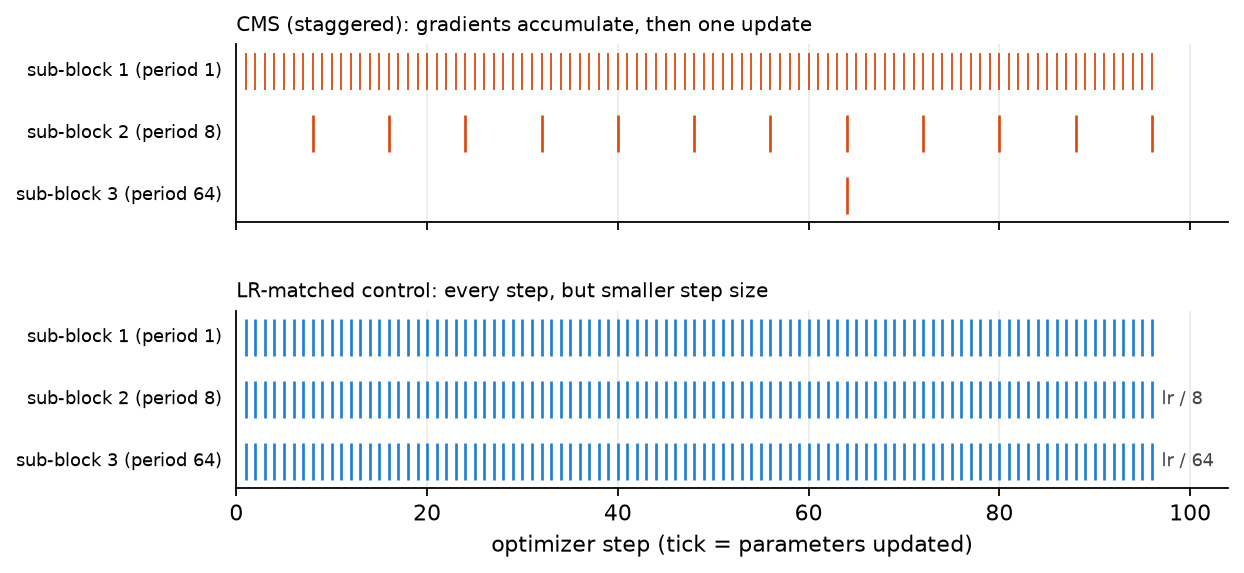
\includegraphics[width=0.78\linewidth]{../figures/update_schedule.png}
\caption{Update schedules over 96 steps. CMS (top) takes rare, larger updates in deeper sub-blocks; the LR-matched control (bottom)
updates every step with a smaller step.}\label{fig:sched}
\end{figure}

\subsection{Forgetting, plasticity and matched comparison}
A model trains on domain 1 (TinyStories) and then domain 2 (Python code). $R[i,j]$ is the held-out loss on domain $j$ after training on domain $i$
(64 windows of 256 tokens per domain). \emph{Forgetting} is $R[2,1]-R[1,1]$; \emph{plasticity} is the new-domain loss $R[2,2]$.
Slower learning trivially forgets less, so arms are compared at equal plasticity: each arm is run at three
learning rates, forgetting is linearly interpolated as a function of new-domain loss for every seed, and evaluated at the median baseline new-domain loss (used only if
it lies inside every arm's range). Differences are seed-paired with 10{,}000-resample bootstrap 95\% confidence intervals.

\subsection{Pre-registration}
Hypotheses, metrics, thresholds and the decision gate were committed to the repository before the first run (tag \texttt{prereg-v1}); the revised
pilot (\texttt{prereg-pilot-rev1}) and the test-time probe (\texttt{prereg-stage1b}) were declared and tagged before their runs. The practical bar was a
$\geq10\%$ relative reduction in forgetting with the CI below zero and new-domain loss within 2\%. A Holm correction was also pre-registered but never applied: no comparison passed the
unadjusted criterion, and a correction can only make results less significant.
The decision gate: if CMS did not beat the LR-matched control, run a shortened plan. The revised pilot
was declared the final input to that gate.

\section{Experiments and results}
\textbf{Setup.} Domain 1 is the first documents of the TinyStories training file, domain 2 is Python source (codeparrot-clean-valid), streamed over
HTTP and tokenized with GPT-2 BPE. Three seeds (0--2) per configuration on one laptop RTX 3050 (4\,GB); about 9 GPU-hours in total,
8--10\,min per training run. Raw per-run files and every figure's generating script are in the repository.

\subsection{Pilot 1: one learning rate}
Sixteen-million-parameter model, learning rate $6\times10^{-4}$. Table~\ref{tab:p1}: plasticity is matched (within 1\%), and CMS forgets more, not
less. Throughput is unchanged, because gradients are still computed every step, and only 92\% of parameters update per step, so staggering gives no compute saving here.

\begin{table}[h]\centering\small
\begin{tabular}{lcccc}\toprule
Arm & Forgetting (nats) & New-domain loss & Tokens/s & Params updated/step\\\midrule
Baseline & $3.549\pm0.189$ & $2.806\pm0.009$ & 35.7k & 1.000\\
CMS 1/8/64 & $3.726\pm0.100$ & $2.795\pm0.009$ & 36.9k & 0.919\\
LR-matched & $3.622\pm0.043$ & $2.786\pm0.013$ & 36.7k & 1.000\\\bottomrule
\end{tabular}
\caption{Pilot 1 (mean $\pm$ sd over 3 seeds). CMS minus baseline: $+0.178$ [$+0.025,+0.334$]; CMS minus LR-matched: $+0.104$ [$+0.026,+0.179$].}\label{tab:p1}
\end{table}

Both pre-registered criteria failed. Weaknesses were visible: the staggered blocks held only about 13\% of the parameters (embeddings are $\sim$80\%),
one learning rate, one domain order, and 3 seeds.

\subsection{Revised pilot: matched plasticity, larger staggered share}\label{sec:pilot2}
The revision (declared before running, with no further revisions allowed) enlarges the staggered share to 39\% (6 layers, $4d$ sub-blocks),
runs every arm at three learning rates ($3\times10^{-4}$, $6\times10^{-4}$, $1.2\times10^{-3}$), and adds a reversed domain order at the middle learning rate: 36 runs.

\begin{table}[h]\centering\small
\begin{tabular}{lccc}\toprule
lr & Baseline & CMS 1/8/64 & LR-matched\\\midrule
$3\times10^{-4}$ & 3.002, 3.172 & 2.978, 3.285 & 2.980, 3.232\\
$6\times10^{-4}$ & 2.802, 3.568 & 2.743, 3.780 & 2.754, 3.632\\
$1.2\times10^{-3}$ & 2.659, 4.007 & 2.588, 4.260 & 2.597, 4.069\\\bottomrule
\end{tabular}
\caption{Revised pilot, order A: (new-domain loss, forgetting in nats), mean of 3 seeds.}\label{tab:p2}
\end{table}

At every learning rate CMS learns the new domain slightly better and forgets slightly more, so the three arms lie on essentially the same
stability--plasticity line (Figure~\ref{fig:front}). At the matched new-domain loss of 2.79 (inside every arm's range for every seed):
baseline $3.592\pm0.163$, CMS $3.678\pm0.060$, LR-matched $3.567\pm0.049$. CMS minus baseline: $+0.085$ [$-0.169,+0.252$] ($+2.4\%$);
CMS minus LR-matched: $+0.111$ [$-0.013,+0.179$] ($+3.1\%$); LR-matched minus baseline: $-0.025$ [$-0.156,+0.085$]. Neither bar was met, so the pre-registered gate selected the shortened plan.
The reversed order (lr $6\times10^{-4}$) agrees: baseline $4.90\pm0.17$, CMS $5.14\pm0.20$, LR-matched $5.20\pm0.07$.

\begin{figure}[t]\centering
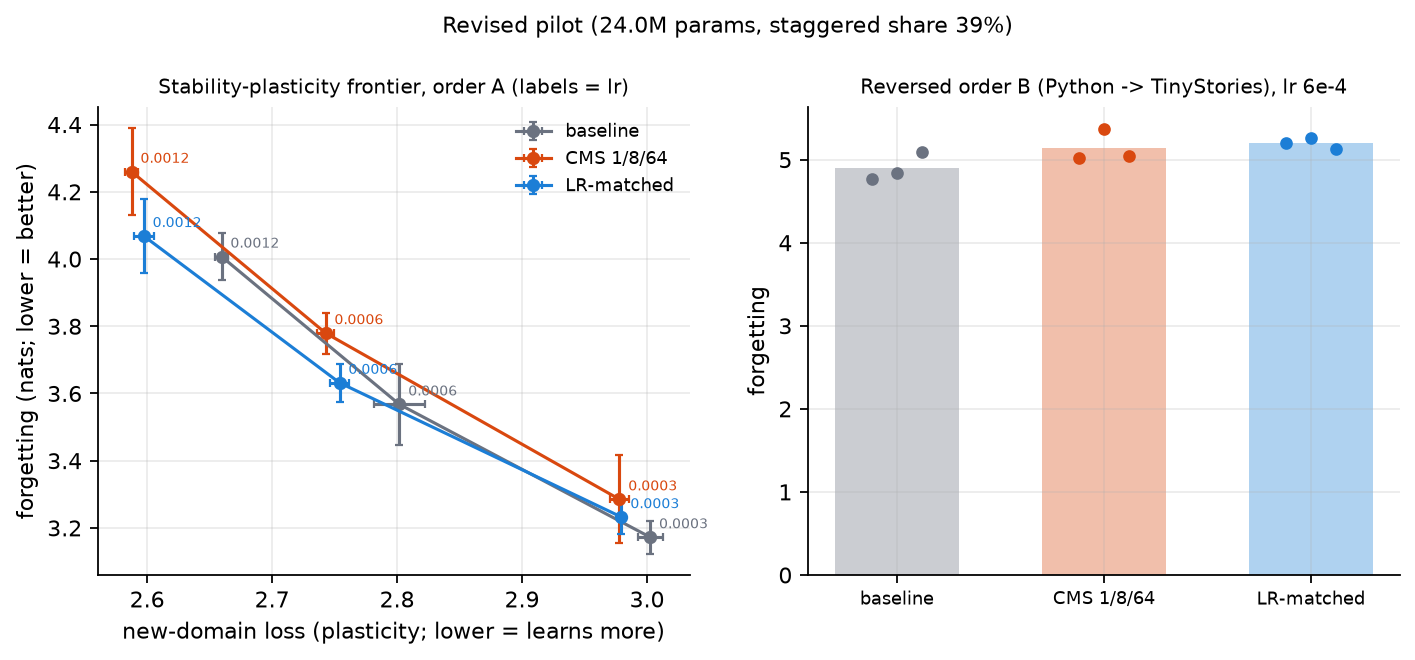
\includegraphics[width=0.92\linewidth]{../figures/pilot_rev_frontier.png}
\caption{Revised pilot. Left: stability--plasticity frontier (labels: learning rate). Right: reversed-order check.}\label{fig:front}
\end{figure}

\subsection{Test-time probe}\label{sec:ttt}
Closer to the paper's mechanism, I trained a base model on TinyStories only and streamed about 1M Python tokens through it
(1000 steps of $4\times256$ tokens), scoring each step before updating, with only the MLP sub-blocks trainable (AdamW, constant rate). Arms: frozen
(no updates; the in-context baseline), single-rate updates, CMS (periods 1/8/64 steps), and LR-matched; learning rates $10^{-4}$, $3\times10^{-4}$, $10^{-3}$; 30 runs.
The frozen model reaches a Python loss of 8.60 and, by construction, has no forgetting; every updating arm beats it at every learning rate (declared sanity check passed).

\begin{table}[h]\centering\small
\begin{tabular}{lccc}\toprule
lr & Single-rate & CMS 1/8/64 & LR-matched\\\midrule
$10^{-4}$ & 2.66 (5.80) & 1.84 (5.80) & 1.70 (5.81)\\
$3\times10^{-4}$ & 3.56 (5.88) & 3.16 (5.79) & 2.85 (5.80)\\
$10^{-3}$ & 4.60 (5.98) & 4.22 (5.92) & 3.89 (5.93)\\\bottomrule
\end{tabular}
\caption{Test-time probe: forgetting in nats (final Python loss in brackets), mean of 3 seeds.}\label{tab:ttt}
\end{table}

\textbf{Declared readout.} Using the same matched-plasticity construction, CMS versus single-rate is $-0.17$ [$-0.74,+0.81$] ($-5\%$; fails), and CMS versus LR-matched is $+0.56$ [$+0.40,+0.70$]
($+21\%$; CMS forgets more; fails). This construction is unreliable here: final Python loss barely varies with learning rate (5.79--5.98) and is not monotone, so the curves are nearly vertical
and interpolation amplifies noise (CMS sd 0.92).
\textbf{Post-hoc, same learning rate} (seed-paired; with 3 seeds the bootstrap has 27 distinct resamples, so intervals are coarse):
CMS forgets $31\%$, $11\%$ and $8\%$ less than single-rate updates at the three learning rates (CIs exclude zero) with equal or better Python loss, matching the direction claimed for CMS.
The LR-matched control, however, forgets $36\%$, $20\%$ and $16\%$ less than single-rate and $8$--$11\%$ less than CMS at every learning rate (Figure~\ref{fig:ttt}). Even the lowest rate forgets 2.7 nats with single-rate
updates, so this grid never reaches a mild regime.

	extbf{Lower learning rates (exploratory follow-up).} I therefore added $10^{-5}$ and $3	imes10^{-5}$ (18 runs, declared and tagged as 	exttt{prereg-stage1b-low} before running; no gate).
Forgetting (final Python loss) is 0.85 (5.92), 0.50 (5.95), 0.46 (5.96) for single-rate, CMS and LR-matched at $10^{-5}$, and 1.41 (5.86), 0.91 (5.89), 0.83 (5.89) at $3	imes10^{-5}$.
CMS forgets $41\%$ and $36\%$ less than single-rate; the LR-matched control forgets $8\%$ and $9\%$ less than CMS; all intervals exclude zero, with the same 3-seed caveat. The ordering is unchanged in the milder regime.

\begin{figure}[t]\centering
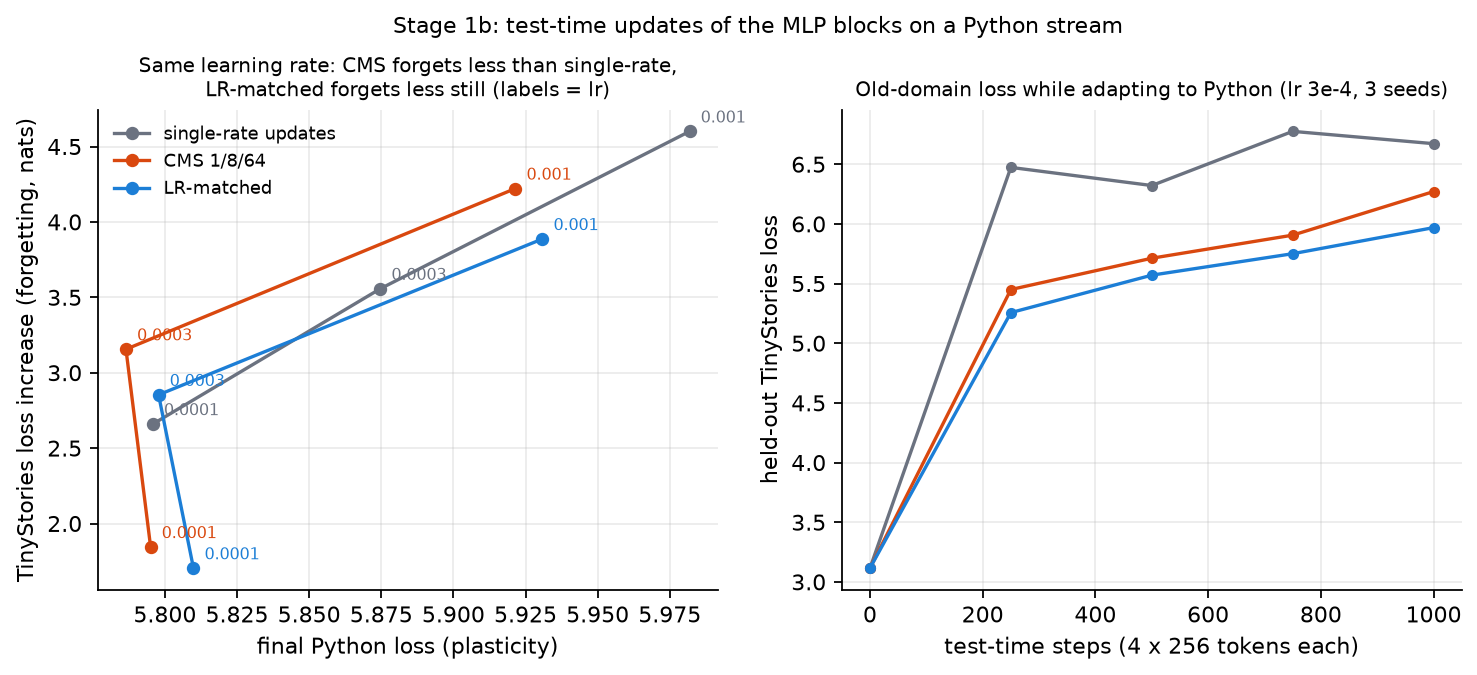
\includegraphics[width=0.95\linewidth]{../figures/ttt_probe.png}
\caption{Test-time probe. Left: forgetting against final Python loss (labels: learning rate). Right: held-out TinyStories loss during the stream (lr $3\times10^{-4}$).}\label{fig:ttt}
\end{figure}

\subsection{Controls and slow momentum (Stage 1c)}\label{sec:s1c}
Declared and tagged (	exttt{prereg-stage1c}) before running; same 24.0M-parameter setup, seeds 0--2, 21 runs. Excess forgetting is read against the baseline frontier at each arm's own new-domain loss.
egin{table}[h]\centering\small
egin{tabular}{llcc}	oprule
Arm & lr & Forgetting & Python loss\\midrule
Baseline & $3	imes10^{-4}$ / $6	imes10^{-4}$ / $1.2	imes10^{-3}$ & 3.17 / 3.57 / 4.01 & 2.69 / 2.49 / 2.37\
Replay (12.5\%) & same & 0.18 / 0.29 / 0.40 & 2.72 / 2.54 / 2.40\
EWC $\lambda=10$ & $6	imes10^{-4}$ & 0.26 & 3.83\
EWC $\lambda=1000$ & $6	imes10^{-4}$ & 0.01 & 4.53\
Slow momentum (± CMS) & $6	imes10^{-4}$ & diverged & 5.0\ottomrule
\end{tabular}
\caption{Stage 1c: forgetting in nats, mean of 3 seeds.}
\end{table}
	extbf{Replay passes the sanity check (H7):} about $90\%$ less forgetting than the baseline frontier ($-3.17$ [$-3.28,-3.09$] and $-3.52$ [$-3.53,-3.50$] at the two higher rates; the lowest rate falls slightly outside the baseline's range, so raw numbers are shown). The benchmark can detect a real remedy, and the effect is about ten times anything seen for staggering.
	extbf{EWC} avoids forgetting by not learning Python (loss 3.8--4.5 against 2.5), so the matched-plasticity readout has no overlap and no claim is made.
	extbf{Slow momentum was unstable as declared} (old-domain loss in the thousands after domain 2; domain 1 already trained worse, 3.48 against 3.13), so H3 and H4 are not assessed. A post-hoc check (seed 0, not pre-registered) that resets optimizer state at the domain boundary did not fix it, while plain AdamW with the same reset behaved normally; I did not find the cause and did not tune the declared constants. This tests my variant (no orthogonalisation) at one learning rate, not M3.

\subsection{Post-hoc diagnostic: where does the movement happen?}
To explain the null, I saved checkpoints after each domain and measured relative weight drift $\|\theta_2-\theta_1\|/\|\theta_1\|$ per parameter group (baseline: 3 seeds; CMS and LR-matched: 1 seed each).
Staggering does what it should: sub-block 3 moves $0.13$ (CMS) and $0.01$ (LR-matched) against $0.62$ for the baseline, sub-block 2 moves $0.22$ and $0.10$ against $0.64$.
Yet forgetting is $3.71$ and $3.60$ against $3.58$. The parts that update every step (embeddings $0.75$--$0.77$, attention $0.55$--$0.58$, first sub-block $0.62$--$0.65$) move equally in every arm.

\begin{figure}[t]\centering
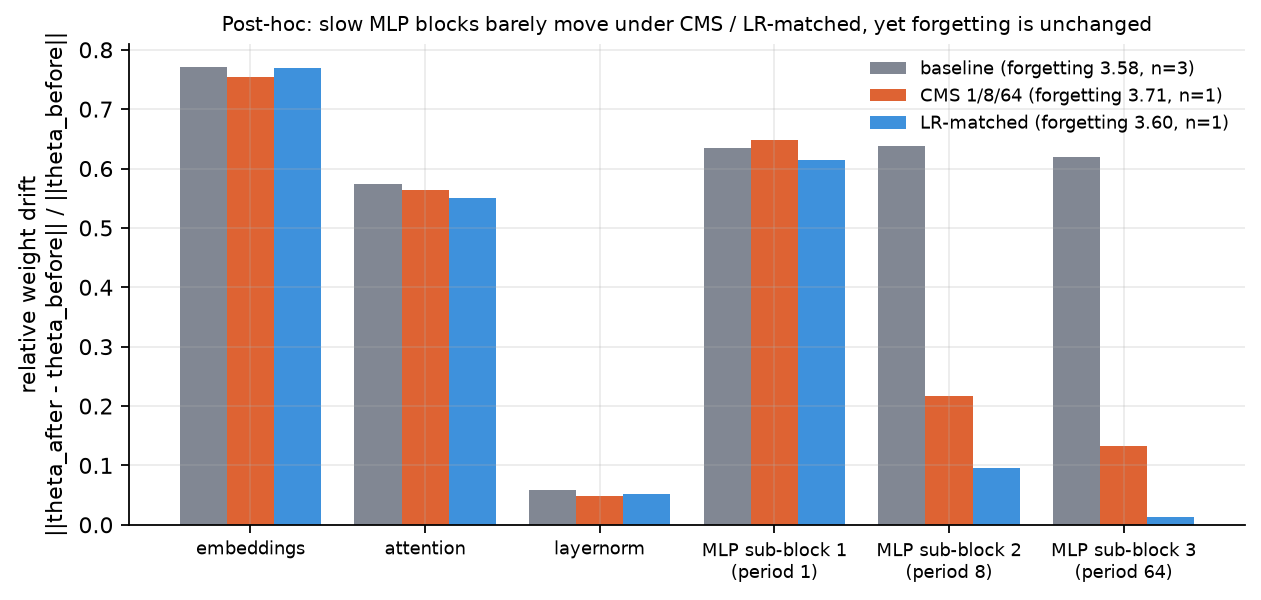
\includegraphics[width=0.88\linewidth]{../figures/drift_diagnostic.png}
\caption{Relative weight drift per parameter group during domain-2 training.}\label{fig:drift}
\end{figure}

This is observational: I did not run the counterfactual of freezing the always-updating parts, and a nearly frozen block may simply matter little for the old domain.
A complementary revert test (resetting one group to its domain-1 weights) is not interpretable as localisation: reverting a single group mixes weights from different
training states and mostly \emph{worsens} old-domain loss; only reverting the embeddings recovers 32--41\% of the forgetting, at the cost of losing the new domain.

\section{Discussion and limitations}
\textbf{What the evidence supports.} Per-step update-frequency staggering in training is not distinguishable from a smaller learning rate, and gives no
forgetting benefit over a normal model at matched plasticity, at 16--24M parameters. At test time, staggering helps relative to updating all blocks at once,
but giving the deeper blocks a smaller step does at least as well. The drift analysis suggests why: the forgetting lives in the parts of the network
that update on every step.

\textbf{What it does not show.} This is not a test of Hope. Untested: nested consolidation between levels (slower levels learning from faster ones),
the self-modifying memory, multi-timescale momentum (the pre-registered slow-momentum arm and the $2\times2$ factorial, hypotheses H3 and H4, were not run), pretrained backbones,
15B-token continual pre-training, and the LoRA stage. The shortened plan the gate selected (replay, EWC, joint-training and in-context baselines at five seeds) was also not run, so no comparison with
standard continual-learning controls is made.

\textbf{Limitations.}
\emph{Small scale and few seeds:} 3 seeds, one period set, $\leq$24M parameters, two domains; bootstrap intervals with 3 seeds are coarse.
\emph{Nondeterminism:} re-running a seed does not reproduce the loss matrix. After domain 1 reruns agree to 0.002 nats, but forgetting after domain 2 differs by $-0.09$ to $+0.11$ nats
between same-seed runs (5 reruns), comparable to the CMS-versus-baseline differences. The CIs include this noise, and the 10\% bar ($\sim$0.36 nats) is well above it, but effects below roughly 0.1 nats are not resolvable per run.
\emph{Implementation details:} the global step counter, and hence the CMS update phase, continues across the domain boundary without flushing partially accumulated gradients (up to 16 steps of the period-64 block's accumulation carry into domain 2),
and optimizer state is not reset between domains. \emph{Regime:} 2000 full-rate steps with no replay raise old-domain loss by more than 3 nats, an extreme regime where mild interventions may be swamped; the first pilot's 10M-parameter target became 16.1M because GPT-2 embeddings dominate.
\emph{Construction:} the matched-plasticity interpolation failed in the test-time probe, and the per-learning-rate comparison there is post-hoc. The base model is not co-trained with staggered blocks.
\emph{Analysis choices:} the drift and revert diagnostics were not pre-registered.

\section{Conclusion}
Across two pre-registered training-time pilots and a test-time probe, staggering update frequencies behaved like a smaller learning rate and did not reduce
catastrophic forgetting beyond what an LR-matched control achieves. The effect that does appear, staggering beating single-rate test-time updates, disappears against the control. I take this as evidence that the
active ingredient in Hope, if there is one, lies elsewhere: in nested consolidation, in the self-modifying memory, or in scale. The most informative next experiments are a CMS-co-trained base with consolidation between levels,
more seeds, and a stable multi-timescale-momentum implementation.

\begin{thebibliography}{99}\small
\bibitem{nl} A.~Behrouz et al. Nested Learning: The Illusion of Deep Learning Architecture. NeurIPS 2025. arXiv:2512.24695.
\bibitem{kmccleary} K.~McCleary. \emph{nested\_learning}: a mechanism-level reproduction of Nested Learning (Hope). \url{https://github.com/kmccleary3301/nested_learning}.
\bibitem{titans} G.~Di Nepi, F.~Siciliano, F.~Silvestri. Titans Revisited: A Lightweight Reimplementation and Critical Analysis of a Test-Time Memory Model. arXiv:2510.09551.
\bibitem{spurious} Spurious Forgetting in Continual Learning of Language Models. ICLR 2025. arXiv:2501.13453.
\bibitem{resampling} How Weight Resampling and Optimizers Shape the Dynamics of Continual Learning and Forgetting in Neural Networks. arXiv:2507.01559.
\bibitem{mech} Mechanistic Analysis of Catastrophic Forgetting in Large Language Models During Continual Fine-tuning. arXiv:2601.18699 (preprint, not independently verified).
\bibitem{fastslow} Learning, Fast and Slow: Towards LLMs That Adapt Continually. arXiv:2605.12484.
\bibitem{clbench} P.~Asawa et al. Continual Learning Bench: Evaluating Frontier AI Systems in Real-World Stateful Environments. arXiv:2606.05661.
\bibitem{trace} TRACE: A Comprehensive Benchmark for Continual Learning in Large Language Models. arXiv:2310.06762.
\bibitem{slao} Merge before Forget: A Single LoRA Continual Learning via Continual Merging. arXiv:2512.23017.
\end{thebibliography}

\appendix
\section{Reproducibility and deviations}
Pre-registration, declarations and deviations log: \texttt{docs/PREREGISTRATION.md}; results log: \texttt{docs/RESULTS.md}; raw runs: \texttt{results/}. Tags
\texttt{prereg-v1}, \texttt{prereg-pilot-rev1}, \texttt{prereg-stage1b} mark each design before its runs. Logged deviations: pilot model 16.1M instead of $\sim$10M parameters; batches run as two micro-batches (identical gradient) to fit 4\,GB;
data streamed over HTTP because pandas/pyarrow are blocked on the development machine; reproducibility check (same seed, same loss matrix) failed because of GPU nondeterminism.
All figures regenerate with \texttt{python scripts/make\_figures.py}.
\end{document}
